%%%%%%%%%%%%%%%%%%%%%%%%%%%%%%%%%%%%%%%%%
% a0poster Portrait Poster
% LaTeX Template
% Version 1.0 (22/06/13)
%
% The a0poster class was created by:
% Gerlinde Kettl and Matthias Weiser (tex@kettl.de)
% 
% This template has been downloaded from:
% http://www.LaTeXTemplates.com
%
% License:
% CC BY-NC-SA 3.0 (http://creativecommons.org/licenses/by-nc-sa/3.0/)
%
%%%%%%%%%%%%%%%%%%%%%%%%%%%%%%%%%%%%%%%%%

%----------------------------------------------------------------------------------------
%	PACKAGES AND OTHER DOCUMENT CONFIGURATIONS
%----------------------------------------------------------------------------------------

\documentclass[a0,portrait]{a0poster}

% increase some sizes
\renewcommand{\footnotesize}{\fontsize{20.74}{25}\selectfont}
\renewcommand{\small}{\fontsize{24.88}{30}\selectfont}
\renewcommand{\normalsize}{\fontsize{29.86}{37}\selectfont}

\usepackage{multicol} % This is so we can have multiple columns of text side-by-side
\columnsep=100pt % This is the amount of white space between the columns in the poster
\columnseprule=1pt % This is the thickness of the black line between the columns in the poster

\usepackage[svgnames]{xcolor} % Specify colors by their 'svgnames', for a full list of all colors available

\usepackage{times} % Use the times font
%\usepackage{palatino} % Uncomment to use the Palatino font

\usepackage{graphicx} % Required for including images
\graphicspath{{./figures/}} % Location of the graphics files
\usepackage{booktabs} % Top and bottom rules for table
\usepackage[font=small,labelfont=bf]{caption} % Required for specifying captions to tables and figures
\usepackage{amsfonts, amsmath, amsthm, amssymb} % For math fonts, symbols and environments
\usepackage{wrapfig} % Allows wrapping text around tables and figures

\usepackage{algorithm}
\usepackage[noend]{algpseudocode}
\usepackage{enumitem}      % adjust spacing in enums
%\usepackage{subfig}
\usepackage{caption}
\usepackage{subcaption}
\usepackage{multirow}
\usepackage{rotating}
\usepackage{balance}
\usepackage{adjustbox}

\usepackage{pgfplots}
% options for pgfplots
\pgfplotsset{compat=1.8,compat/show suggested version=false}
\usetikzlibrary{plotmarks}
\usetikzlibrary{calc}
%\pgfplotsset{compat=newest}
\pgfplotsset{
   /pgfplots/bar  cycle  list/.style={/pgfplots/cycle  list={%
        {black,fill=black!30!white,mark=none},%
        {black,fill=red!30!white,mark=none},%
        {black,fill=green!30!white,mark=none},%
        {black,fill=yellow!30!white,mark=none},%
        {black,fill=brown!30!white,mark=none},%
     }
   },
}
% begin of externalization
\usetikzlibrary{external}
\tikzexternalize[prefix=./out/]
\tikzexternalize 
% don't externalize todonotes
%\makeatletter
%\renewcommand{\todo}[2][]{\tikzexternaldisable\@todo[#1]{#2}\tikzexternalenable}
%\makeatother
% end of externalization
\usetikzlibrary{patterns}
\usepgfplotslibrary{groupplots}
\pgfplotsset{
every axis label/.append style={font=\small},
tick label style={font=\small},
}

% \pdfstringdefDisableCommands{
%     \def\\{}
%     \def\unskip{}
%     \def\texttt#1{<#1>}
% }

\DeclareCaptionFormat{subfig}{\figurename~#1#2#3}
\DeclareCaptionSubType*{figure}
\captionsetup[subfigure]{format=subfig,labelsep=colon,labelformat=simple}

%\newcommand{\comment}[[1]{\textcolor{red}{#1}}
\newcommand{\myworries}[1]{\textcolor{red}{#1}}
\newcommand{\cutout}[1]{}
\newcommand{\smallcaption}[1]{\caption[#1]{{\protect\small \protect\bf #1}}}
\newcommand{\dids}{{\sc dids}}

% some useful shortcuts
\newcommand{\ie}{\textit{i.e., }}
\newcommand{\eg}{\textit{e.g., }}
\newcommand{\CC}{C\nolinebreak\hspace{-.05em}\raisebox{.5ex}{\tiny\bf +}\nolinebreak\hspace{-.10em}\raisebox{.5ex}{\tiny\bf +}}

% units for results
\newcommand{\us}{\,$\mu$s}
\newcommand{\ms}{\,ms}
\newcommand{\KB}{\,KB}
\newcommand{\MB}{\,MB}
\newcommand{\GB}{\,GB}
\newcommand{\MHz}{\,MHz}
\newcommand{\GHz}{\,GHz}

\newcommand{\PAD}{\vskip 0.75cm}

% new latex commands:
%   Remove long section
\newcommand{\PUNT}[1]{}
\newcommand{\TABLETWO}[1]{}
%   Label work to be done
\definecolor{gray}{gray}{0.75}
\newcommand{\TODO}[1]{\textcolor{gray}{\textbf{\ [TODO:\ #1]\ }}}
\newcommand{\TR}[1]{#1}
%\newcommand{\TR}[1]{}
%\newcommand{\TODO}[1]{}
\newcommand{\FIX}[1] {\textcolor{red}{\textbf{\ [FIX:\ #1]\ }}}
%   Referencing various pieces of the document:
\newcommand{\figref}[1]{Fig.~\ref{fig:#1}}
\newcommand{\figsref}[2]{Figures~\ref{fig:#1} and~\ref{fig:#2}}
\newcommand{\figrref}[2]{Figures~\ref{fig:#1}--\ref{fig:#2}}
\newcommand{\secref}[1]{Section~\ref{sec:#1}}
\newcommand{\secsref}[2]{Sections~\ref{sec:#1} and~\ref{sec:#2}}
\newcommand{\eqnref}[1]{Eqn.~\ref{eqn:#1}}
\newcommand{\eqnsref}[2]{Equations~\ref{eqn:#1} and~\ref{eqn:#2}}
\newcommand{\eqnrref}[2]{Equations~\ref{eqn:#1}--\ref{eqn:#2}}
\newcommand{\insref}[1]{Instruction~\ref{ins:#1}}
\newcommand{\tblref}[1]{Table~\ref{tbl:#1}}
\newcommand{\appref}[1]{Appendix~\ref{app:#1}}

\newcommand{\algoref}[1]{Algorithm~\ref{algo:#1}}

% Custom hyphenation rules

%\DeclareMathOperator{\minimize}{minimize}
%\DeclareMathOperator{\st}{s.t.}
%\DeclareMathOperator*{\argmin}{arg\,min}
%\DeclareMathOperator*{\argmax}{arg\,max}
\newcommand{\argmin}{\arg\!\min}
\newcommand{\argmax}{\arg\!\max}
\newcommand{\minimize}{minimize}
\newcommand{\optimize}{optimize}
\newcommand{\ceil}[1]{\lceil #1 \rceil}
\newcommand{\floor}[1]{\lfloor #1 \rfloor}
\newcommand{\st}{s.t.}

\usepackage[natbib=true,backend=bibtex,firstinits=true,style=numeric-comp,sorting=nyt,defernumbers,maxnames=2,maxcitenames=2,doi=false,isbn=false,url=false]{biblatex}
\bibliography{strongbox}
\renewcommand*{\bibfont}{\normalfont\footnotesize}

\begin{document}

%----------------------------------------------------------------------------------------
%	POSTER HEADER 
%----------------------------------------------------------------------------------------

% The header is divided into two boxes:
% The first is 75% wide and houses the title, subtitle, names, university/organization and contact information
% The second is 25% wide and houses a logo for your university/organization or a photo of you
% The widths of these boxes can be easily edited to accommodate your content as you see fit

\begin{minipage}[b]{\linewidth}

\includegraphics[height=5cm]{figures/strongbox_logo}\hspace*{0.25cm}

\includegraphics[height=5cm]{figures/uchicago_logo}
\vspace{0.1cm}
\begin{center}
\noindent\makebox[\linewidth]{\rule{0.9\paperwidth}{0.4pt}}
\vspace{0.1cm}
\end{center}

\veryHuge \color{NavyBlue} \textbf{Strongbox: Fast Secure Storage for Mobile Devices} \color{Black}\\[0.5cm] % Title
% \Huge\textit{An Exploration of Complexity}\\[2cm] % Subtitle
\huge \textbf{Bernard Dickens, Ariel Feldman, Haryadi Gunawi, Henry Hoffmann}\\[0.25cm] % Author(s)
\Large University of Chicago %//[0.25cm] % University/organization
% \Large \texttt{bd3@cs.uchicago.edu}\\
\end{minipage}

\vspace{1cm} % A bit of extra whitespace between the header and poster content

%----------------------------------------------------------------------------------------

\begin{multicols}{2} % This is how many columns your poster will be broken into, a portrait poster is generally split into 2 columns

%----------------------------------------------------------------------------------------
%	ABSTRACT
%----------------------------------------------------------------------------------------

\color{Navy} % Navy color for the abstract

\begin{abstract}

Full disk encryption (FDE) is especially important for mobile devices because
they both contain large amounts of sensitive data and are easily lost or stolen.
Yet, the conventional approach to FDE, AES in XTS mode, is 3--5x slower than
unencrypted storage. Authenticated encryption based on stream ciphers like
ChaCha20 is already used as a faster alternative to AES in other contexts, such
as HTTPS, but the conventional wisdom is that stream ciphers are a unsuitable
for FDE. Used naively in disk encryption, stream ciphers are vulnerable to
many-time pad attacks and rollback attacks, and mitigating these attacks with
on-disk metadata is generally believed to ruin performance.

In this paper, we argue that recent developments in mobile devices invalidate
this assumption and make it possible to use fast stream ciphers for disk
encryption. Modern mobile devices rely on NAND-flash storage with a Flash
Translation Layer (FTL), which functions very similarly to a Log-structured File
System (LFS), and include trusted hardware such as Trusted Execution
Environments (TEEs) and secure storage areas. Leveraging these two trends, we
propose StrongBox, a stream cipher-based FDE layer that is a drop-in replacement
for dm-crypt, the standard Linux disk encryption module based on AES-XTS.
StrongBox introduces a system design and on-disk data structures that exploit
LFS's lack of overwrites to avoid costly rekeying and a counter stored in
trusted hardware to implement rollback protection. We implement StrongBox on an
ARM big.LITTLE mobile processor and test its performance under the F2FS LFS.

\end{abstract}

%----------------------------------------------------------------------------------------
%	INTRODUCTION
%----------------------------------------------------------------------------------------

\color{SaddleBrown} % SaddleBrown color for the introduction

\section*{Motivation}

Full disk encryption (FDE) is an essential technique for protecting the privacy
of data at rest. Considering the state of the art, the conventional wisdom for
securing this data is to use the AES block cipher in XTS mode~\cite{NISTXTS}.
Potentially more performant steam ciphers are not typically considered.

However, technological shifts in mobile devices overturn this conventional
wisdom and make it possible to use more performant stream ciphers for disk
encryption. First, mobile devices commonly use Flash Translation Layers (FTL)
and/or Log-structured File Systems (LFSes)~\cite{LFS,F2FS,NILFS} to increase the
lifetime of their solid-state drives (SSDs). Second, modern mobile devices like
smartphones now come equipped with trusted hardware~\cite{TEE,TrustZone}, such
as Trusted Execution Environments (TEEs) and secure storage
areas~\cite{eMMC-standard}.

We demonstrate the potential performance win from switching to a stream cipher
by comparing AES-XTS to ChaCha20+Poly1305. \figref{motivation} shows the
distinct advantage of the stream cipher over AES: a consistent $2.7\times$
reduction in run time.

We believe stream ciphers are best suited for encrypting block devices backing
Log-structured File Systems, as these filesystems are designed to append data to
the end of a log rather than over-write data. In practice, some overwrites
occur; \eg{in metadata}, but they are small in number during normal execution.
This motivates our approach of using a stream cipher to perform full disk
encryption under Log-structured File Systems.

\vspace{0.5cm}

\begin{minipage}{\columnwidth}
\PAD 
\begin{tikzpicture}

\begin{groupplot}[
    group style={
        group name=plots,
        group size=1 by 1,
        xlabels at=edge top,
        xticklabels at=edge top,
        vertical sep=5pt
    },
axis x line* = top,
xlabel near ticks,
major x tick style = transparent,
height=5cm,
%width=0.95\columnwidth,
width=0.9\columnwidth,
xmin=0,
xmax=3,
enlargelimits=false,
tick align = outside,
tick style={white},
ytick=\empty,
xtick=\empty,
xticklabels={},
yticklabels={},
]
\nextgroupplot[ylabel={\scriptsize Time (s)},
ylabel shift={6mm},
ymin=0,
ymax=1,
]


\end{groupplot}

\begin{groupplot}[
    group style={
        group name=plots,
        group size=1 by 1,
        xlabels at=edge bottom,
        xticklabels at=edge bottom,
        vertical sep=5pt
    },
axis x line* = bottom,
xlabel near ticks,
major x tick style = transparent,
height=5cm,
%width=0.95\columnwidth,
width=0.9\columnwidth,
xmin=0,
xmax=3,
enlargelimits=false,
tick align = outside,
tick style={white},
ytick=\empty,
xticklabel shift={-5pt},
%x tick label style={rotate=0, anchor=south},
%xlabel={\footnotesize $Platform$}
xtick={1,2},
xticklabels={{\scriptsize $\mathsf{Encrypt}$},
{\scriptsize $\mathsf{Decrypt}$}},
ymin=0,
ymax=50,
ytick={0,12.5,25,37.5,50},
yticklabels={\scriptsize{0},,\scriptsize{25},,\scriptsize{50}},
legend cell align=left, 
legend style={ column sep=1ex },
ymajorgrids,
grid style={dashed},
]
\nextgroupplot[ybar=\pgflinewidth,
bar width=15pt,
legend entries = {{\scriptsize $\mathsf{AES-XTS}$},
{\scriptsize $\mathsf{ChaCha+Poly1305}$}
},
legend style={draw=none,legend columns=2,at={(0.5,1.35)},anchor=north},
]
\addplot table[x index=0,y index=4, col sep=space] {img/heuristics2.txt};
\addplot table[x index=0,y index=5, col sep=space] {img/heuristics2.txt};


\end{groupplot}

\end{tikzpicture}

\captionof{figure}{AES-XTS and ChaCha20+Poly1305 Comparison.}\label{fig:motivation}
\PAD 
\end{minipage}\\
\begin{minipage}{\columnwidth}
\PAD 
\centering
\begin{tabular}{l|c|c} 
  \small{\textbf{File System}} & \small{\textbf{Total Write Ops}} & \small{\textbf{Overwrites}}  \\
  \hline
  \hline
  ext4    &  16,756 & 10,787\\
  LogFS   &   4,244 &     32\\
  NILFS   &   4,199 &     24\\
  F2FS    &   2.107 &      2\\
  \hline 
  \hline
\end{tabular}
\captionof{table}{File System Overwrite Behavior}\label{tbl:overwrites}
\PAD 
\end{minipage}

\vspace{-1cm}

%----------------------------------------------------------------------------------------
%	OBJECTIVES
%----------------------------------------------------------------------------------------

\color{DarkSlateGray} % DarkSlateGray color for the rest of the content

\section*{StrongBox Design}

StrongBox's design is illustrated in \figref{overview}. StrongBox's metadata---
the key to its operation---is encapsulated in three primary components: an in-
memory \emph{Merkle Tree} and two disk-backed byte arrays, the \emph{Keycount
Store} and the \emph{Transaction Journal}. These components are integrated into
the \emph{Cryptographic Driver}, which is responsible for handling data
encryption, verification, and decryption. These interactions take place while
fulfilling high-level I/O requests received from the overlying LFS.

\begin{minipage}{0.6\columnwidth}
\PAD 
\centering
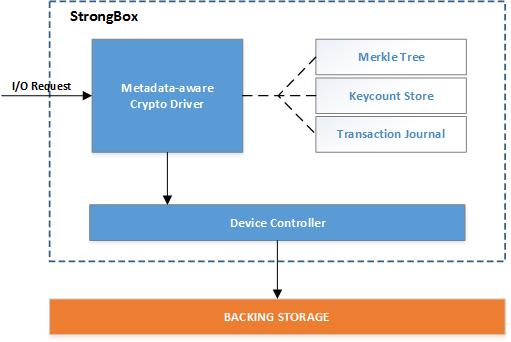
\includegraphics{overview}
\captionof{figure}{Overview of the StrongBox construction.}\label{fig:overview}
\PAD 
\end{minipage}
\begin{minipage}{0.4\columnwidth}
\PAD 
\centering
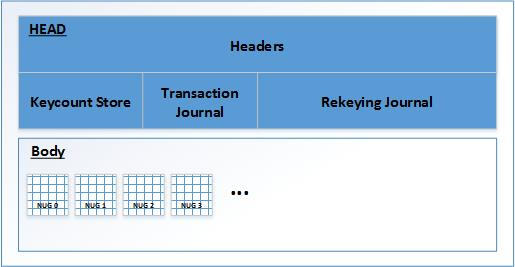
\includegraphics{backstore}
\captionof{figure}{Layout of StrongBox’s backing storage.}\label{fig:backstore}
\PAD 
\end{minipage}

%----------------------------------------------------------------------------------------
%	MATERIALS AND METHODS
%----------------------------------------------------------------------------------------

\section*{StrongBox vs Dm-crypt under F2FS}

To evaluate the performance of StrongBox, we measure the latency
(seconds/milliseconds per operation) of both sequential and random read and
write I/O operations across four different standard Linux filesystems: NILFS2,
F2FS (shown below), Ext4 in ordered journaling mode, and Ext4 in full journaling mode.

We include results of the F2FS LFS mounted atop both dm-crypt and StrongBox;
median latency of different sized whole file read and write operations were
normalized to unencrypted access. By harmonic mean, StrongBox is 1.6$\times$
faster than dm-crypt for reads and 1.3$\times$ faster for writes.

\begin{minipage}{\columnwidth}
\PAD 
\centering
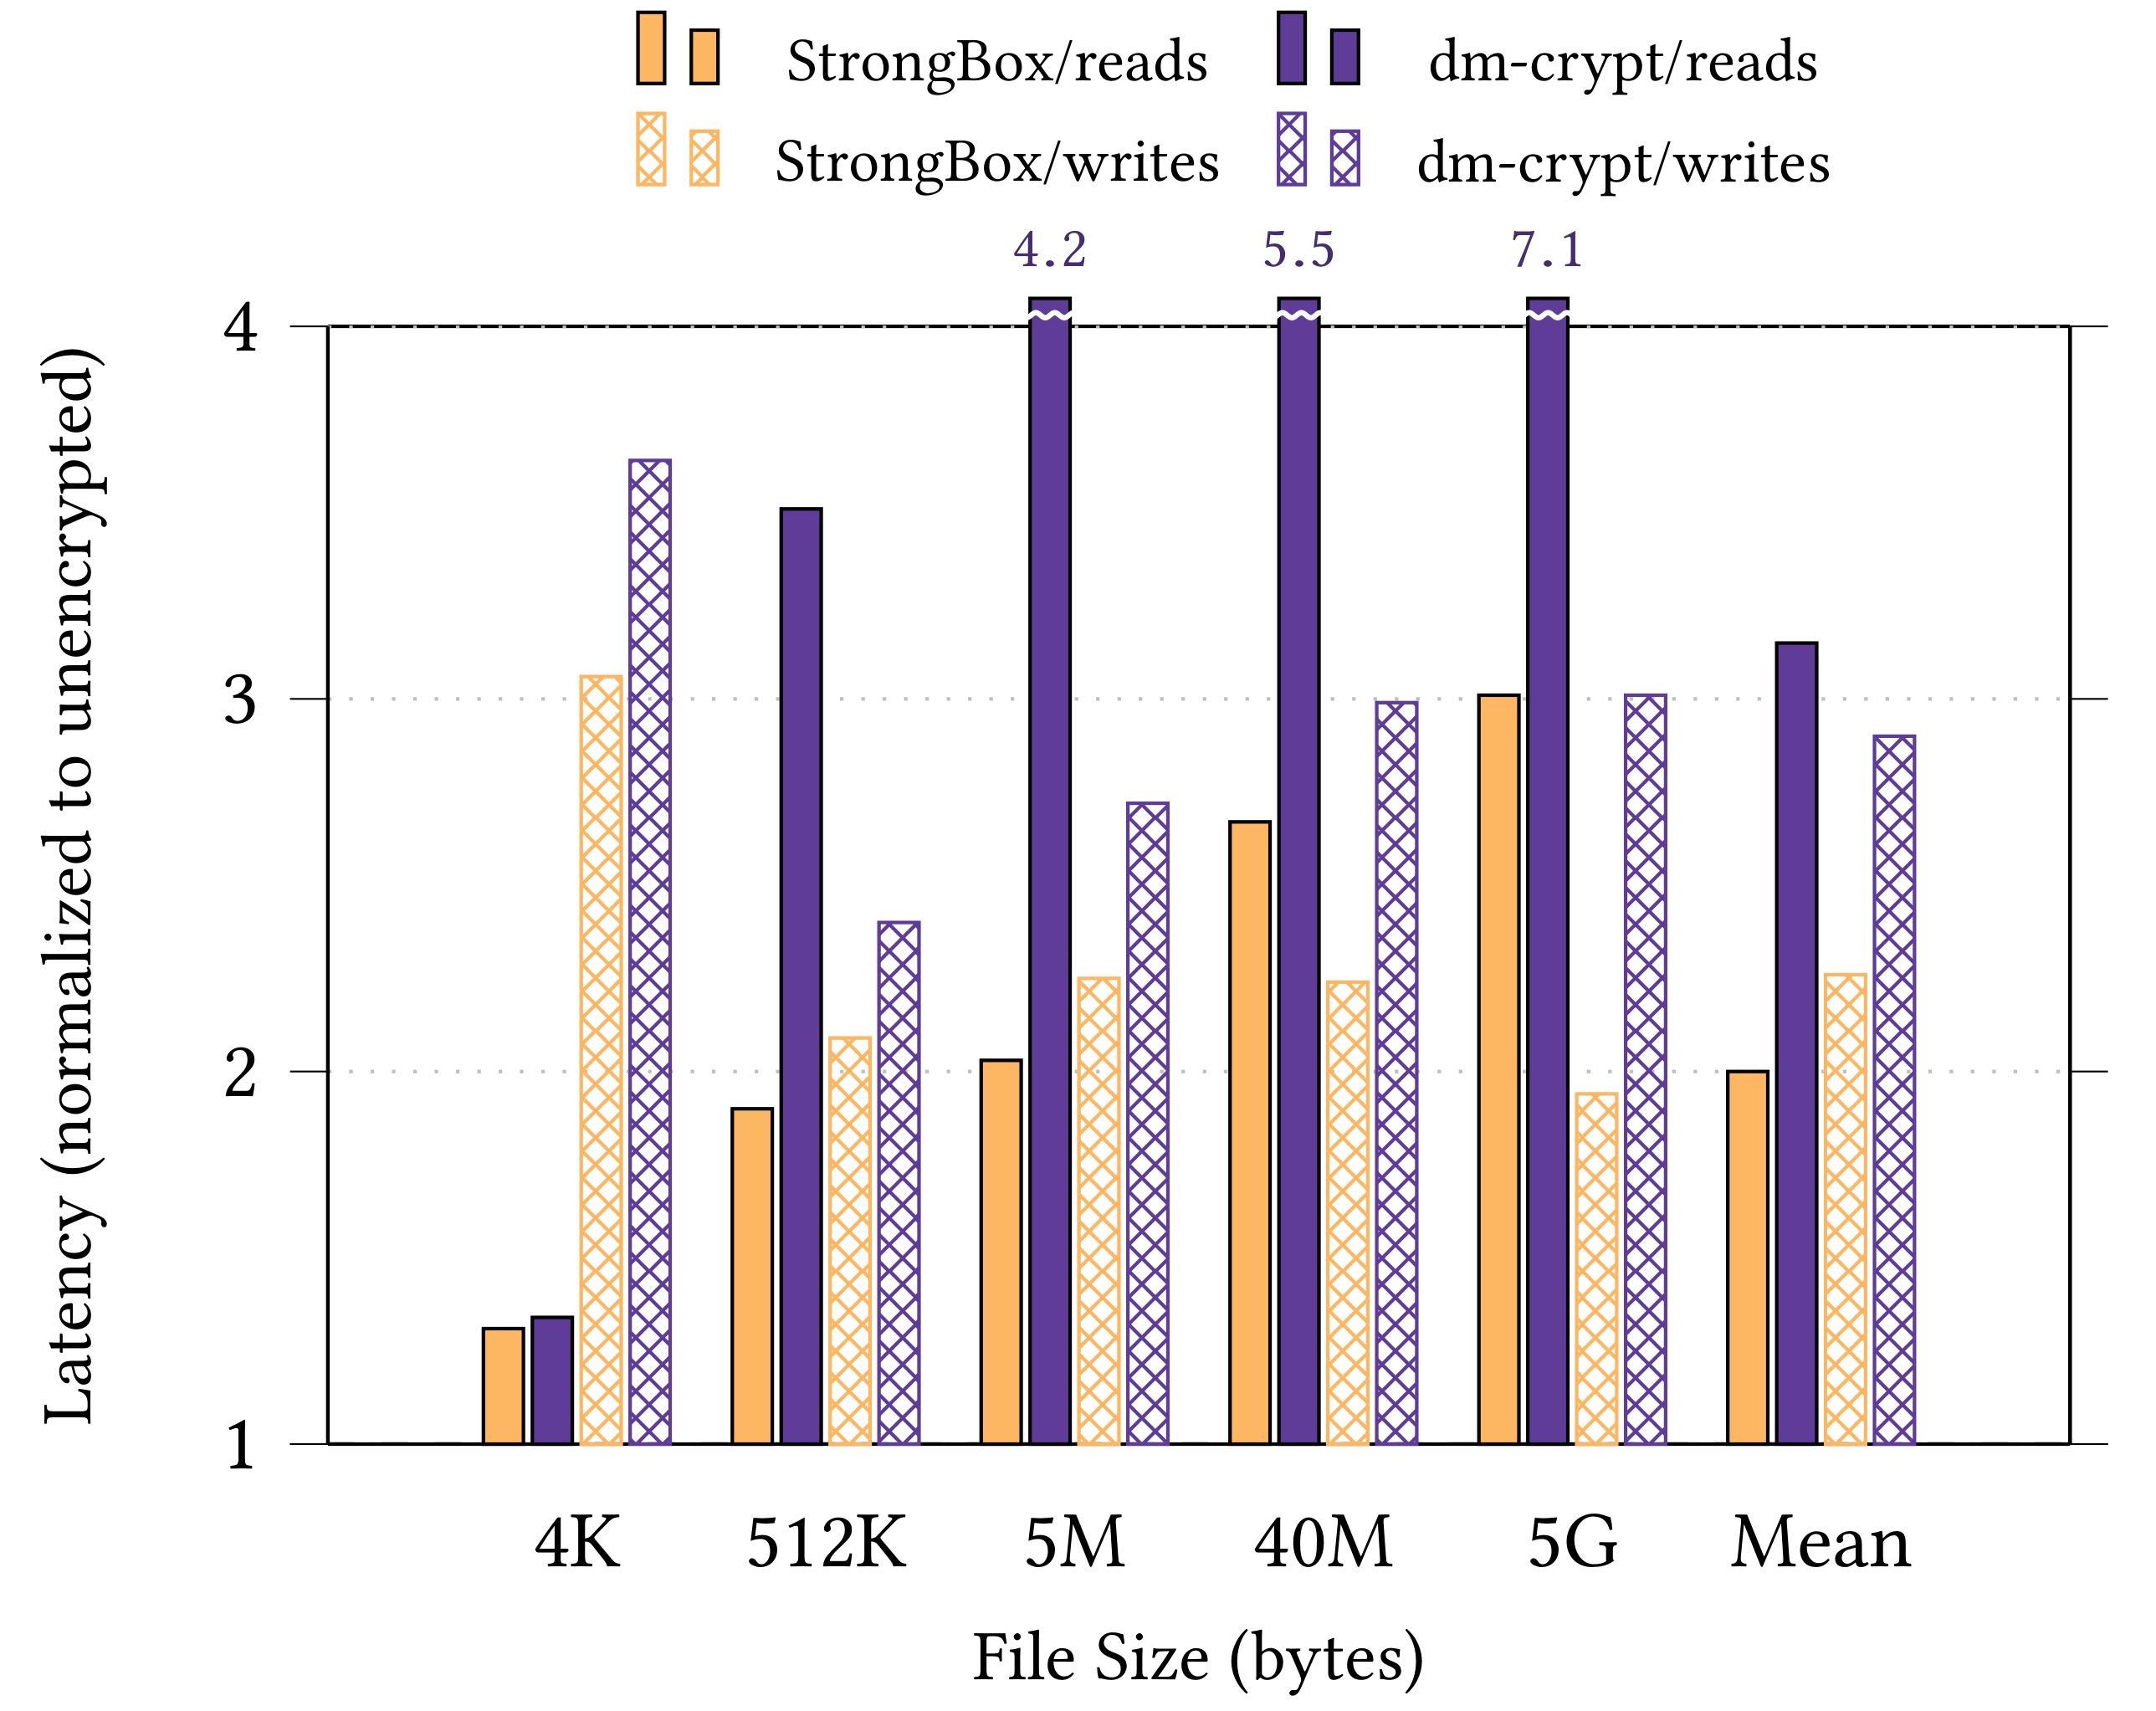
\includegraphics[scale=0.45]{first_bars}
\captionof{figure}{Sequential I/O F2FS result set.}\label{fig:microbench-f2fs-sequential}
\PAD 
\end{minipage}\\[1ex]
\begin{minipage}{\columnwidth}
\PAD 
% \centering
% 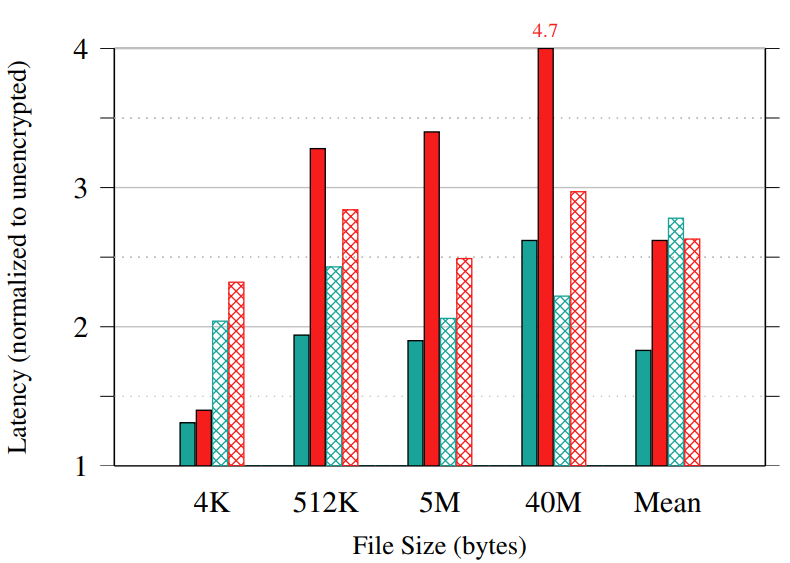
\includegraphics[scale=0.4]{second_bars}
% \captionof{figure}{Sequential I/O FS expanded result set.}\label{fig:microbench-f2fs}
% \PAD 
\end{minipage}

%----------------------------------------------------------------------------------------
%	CONCLUSIONS
%----------------------------------------------------------------------------------------

\color{SaddleBrown} % SaddleBrown color for the conclusions to make them stand out

\section*{Conclusion}

\begin{itemize}

\item The conventional wisdom: securing data at rest requires one must pay the
large performance overhead of encryption with the AES-XTS block cipher instead
of using a stream cipher.

\item The proliferation of NAND-flash FTL/LFS and secure hardware on
modern/mobile devices overturns the conventional wisdom, making it practical to
use a stream ciphers to secure data at rest.

\item We propose StrongBox, a stream cipher-based FDE layer and drop-in
replacement for dm-crypt. StrongBox exploits LFS’s lack of overwrites and the
availability of trusted hardware to overcome the limitations of stream ciphers.

\item Our results show that under F2FS, StrongBox provides upwards of
$2\times$ improvement on read performance and $1.3\times$ improvement on write
performance over a standard dm-crypt configuration.

\end{itemize}

\textcolor{black}{\footnotesize{*StrongBox source is available on GitHub @ \texttt{https://git.xunn.io/research/buselfs-public}}}

\color{DarkSlateGray} % Set the color back to DarkSlateGray for the rest of the content

%----------------------------------------------------------------------------------------
%	REFERENCES
%----------------------------------------------------------------------------------------

% \nocite{*} % Print all references regardless of whether they were cited in the poster or not
\printbibliography 
% \bibliographystyle{plain} % Plain referencing style
% \bibliography{strongbox} % Use the example bibliography file sample.bib

%----------------------------------------------------------------------------------------

\end{multicols}
\end{document}
